\documentclass[10pt]{article}
\usepackage[polish]{babel}
\usepackage[utf8]{inputenc}
\usepackage[T1]{fontenc}
\usepackage{amsmath}
\usepackage{amsfonts}
\usepackage{amssymb}
\usepackage[version=4]{mhchem}
\usepackage{stmaryrd}
\usepackage{graphicx}
\usepackage[export]{adjustbox}
\graphicspath{ {./images/} }

\title{LIGA MATEMATYCZNA \\
 im. Zdzisława Matuskiego \\
 PAŹDZIERNIK 2017 \\
 SZKOŁA PONADGIMNAZJALNA }

\author{}
\date{}


\begin{document}
\maketitle
\section*{ZADANIE 1.}
Oblicz sumę

\[
[\sqrt{1}]+[\sqrt{2}]+[\sqrt{3}]+[\sqrt{4}]+\ldots+\left[\sqrt{n^{2}-1}\right]
\]

gdzie \(n\) jest dowolną liczbą naturalną większą od 1, a symbol \([x]\) oznacza największą liczbę całkowitą nie przekraczającą liczby \(x\).

\section*{ZADANIE 2.}
Rozwiąż równanie

\[
20 a^{2}+10 b^{2}=2010
\]

w zbiorze liczb naturalnych.

\section*{ZADANIE 3.}
Wykaż, że liczba \(201^{8}+3 \cdot 201^{4}-4\) jest podzielna przez 4000.

\section*{ZADANIE 4.}
Wykaż, że każda liczba naturalna większa od 10 jest sumą trzech liczb: dwóch różnych liczb pierwszych i jednej złożonej.

\section*{ZADANIE 5.}
Dany jest trapez \(A B C D\) o podstawach \(a\) i \(b\). Odcinek \(E F\) o długości \(x\) jest równoległy do podstaw trapezu i podzielił go na dwa trapezy o równych polach. Wyznacz \(x\).\\
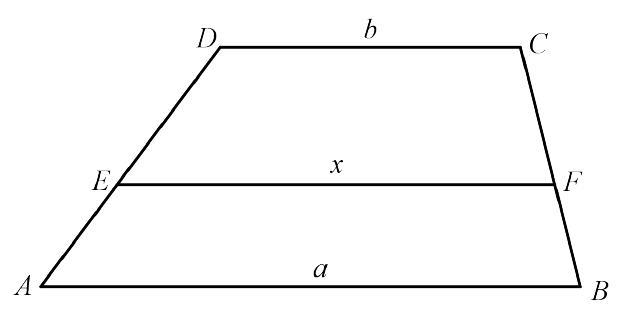
\includegraphics[max width=\textwidth, center]{2024_11_21_41366cd13784fcaf3560g-1}


\end{document}